%=== CHAPTER THREE (3) ===
%=== (Actual work done and contribution, including literature survey) ===

\chapter{Approach}

\section{Quantitative Trajectory Evaluation Method}
To evaluate the mapping performance, the proposed method in \cite{zhang2018tutorial} is modified to multi robot case, and employed in this work.

The previous work of CORB-SLAM in \cite{li2017corb} only provides a rough overview of the mapping result of the multi robot system, as seen in Figure \ref{fig:corbslamresult}.

In \cite{maddern2014illumination} and \cite{arroyo2016openable}, the results of the illumination variance localization are also only briefly introduced, with no quantitative results given.

In this paper, mapping results of CORB-SLAM and CORB-SLAM integrated with illumination variance are evaluated following the quantitative trajectory evaluation method proposed in \cite{zhang2018tutorial}. Quantitative evaluation results of each datasets are demonstrated in several figures and tables including contents as follows, and see Section \ref{sec:kittievaluate} as an example: 

\begin{enumerate}[1.]
	\item Ground truth trajectories of each partial sequence and the complete dataset for reference, e.g. Figure \ref{fig:kittigt}.
	\item Mapping results of each client and fused map in server end, compared with ground truth trajectories, e.g. Figure \ref{fig:kittiresults}.
	\item Four charts of quantitative results, e.g. Figure \ref{fig:kittiquanresult}, including 
	\label{enum:chartsinfo}
	\begin{enumerate}[1).]
		\item Chart of relative translation error in meter, e.g. Figure \ref{sfig:kittireltran}.
		\item Chart of relative translation error in percent, e.g. Figure \ref{sfig:kittireltranper}.
		\item Chart of relative yaw error in degree, e.g. Figure \ref{sfig:kittirelyaw}.
		\item Chart of scale error in percent, e.g. Figure \ref{sfig:kittiscaleerr}.
	\end{enumerate}
	\item A table presenting numeric results of charts in \ref{enum:chartsinfo}, e.g. Table \ref{tbl:kittiquanresult}.
	\item Charts of quantitative results of mapping each partial sequences in each client, in the same format of \ref{enum:chartsinfo}, e.g. Figure \ref{fig:kittiseq0quanresult}.
	\label{enum:clientchartinfo}
	\item A table presenting numeric results of charts in \ref{enum:clientchartinfo}, e.g. Table \ref{tbl:kittiseq0quanresult}.
	\item (if applicable) The mapping results of CORB-SLAM mapping the entire sequence without partial sequences for reference, e.g. Figure \ref{fig:kitticlientmapping}.
	\item (if applicable) Charts of quantitative results of mapping the entire sequence for reference, in the same format of \ref{enum:chartsinfo}, e.g. Figure \ref{fig:kittientirequanresult}.
	\label{enum:refchartinfo}
	\item (if applicable) A table presenting numeric results of charts in \ref{enum:refchartinfo}, e.g. Table \ref{tbl:kitticlientquanresult}.
\end{enumerate}

\begin{figure}[H]
	\centering
	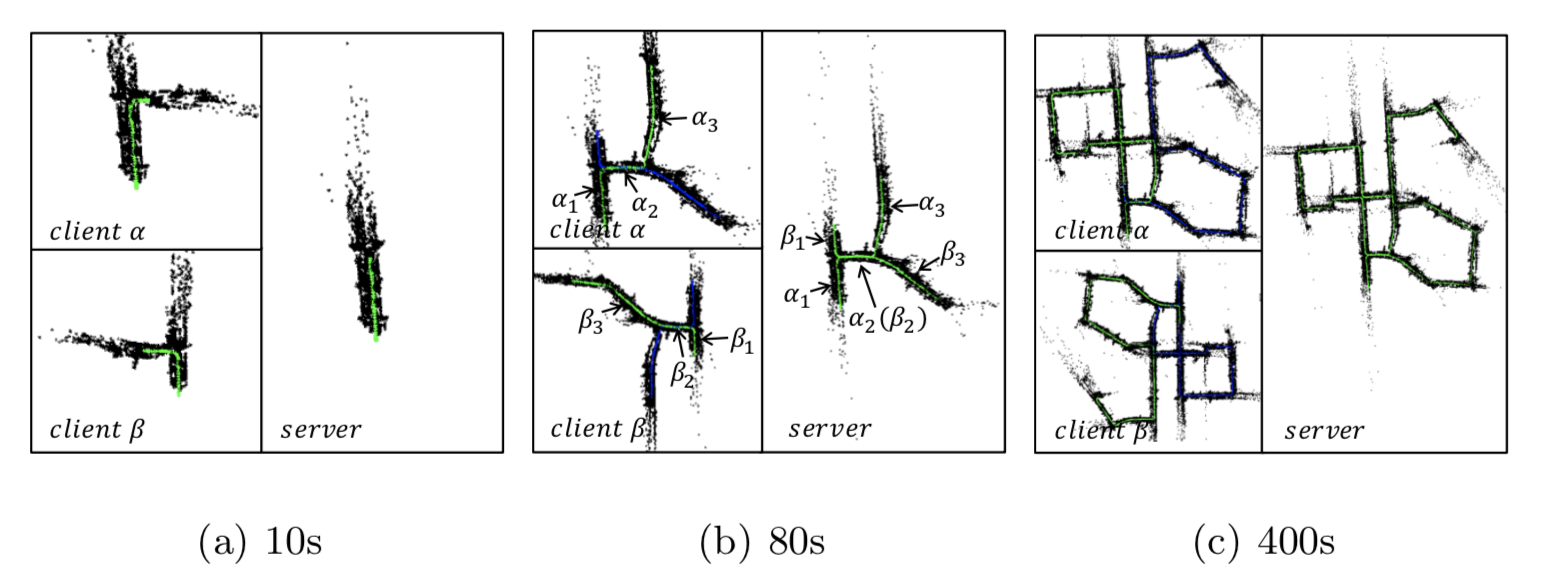
\includegraphics[width=5in]{Chapter3/corbslamresult.eps}
	\caption{Mapping results of CORB-SLAM in \cite{li2017corb}.}
	\label{fig:corbslamresult} 
\end{figure}

The main task of map fusion module of multi robot SLAM server is to find relative relationship including rotation and transformation matrices between client maps, based on which client maps are fused into a consist global map. Therefore, inaccurate rotation and transformation result in an inaccurate fused global map where all client maps but the one set to be the initial global map are stitched dramatically offsetting the ground truth trajectories, which therefore causes serious translation and yaw error. Therefore in charts and tables of quantitative results, three types of relative errors are selected: 
\begin{inparaenum}
	\item Relative Translation Error. \item Relative Translation Error in percent.  \item Relative Yaw Error.
\end{inparaenum}


\section{CORBSLAM with Illumination Variance}

To enhance the ability of CORB-SLAM to map in different illumination conditions and seasons, Illumination Variance method is combined into the map fusion modules of CORB-SLAM server. The block diagram of the integrated system is illustrated in Figure \ref{fig:coislamoverview}.

\begin{figure}[H]
	\centering
	
\includegraphics[width=5in]{thereisafigure.eps}
	\caption{The block diagram of the modified system of CORB-SLAM integrated with illumination variance.}
	\label{fig:coislamoverview} 
\end{figure}

In the client end, the following modifications are made:

\begin{enumerate}
	\item A new thread running in parallel is added to process the input frame to transform into illumination variance images, and extract ORB keypoints in produced images (named as \textsl{II keypoints} in this paper).
	\item II keypoint data is added into each frame as new member variables. And then following the CORB-SLAM methodology, only the integrated keyframes are transmitted to the server,  which are serialized and packed by boost serialization library, and transmitted through ROS service.
\end{enumerate}

Besides the above changes, the following modification are made in the server end:

\begin{enumerate}
	\item A new keydataset containing II keypoint information. 
	\item A new illumination variance localizer running in parallel with the rgb localizer. When processing the input keyframe, a new localizer thread is started if the rgb localizer returns no result. The results from rgb and illumination variance localizer are currently added together in this work.
\end{enumerate}





%=== END OF CHAPTER THREE ===
\newpage
